% \documentclass{beamer}
\documentclass[xcolor=dvipsnames]{beamer}
\usefonttheme{serif}
%% \usecolortheme[named=Blue]{structure}
\setbeamersize{text margin left=30mm, text margin right=30mm}
\useoutertheme{infolines}
%% \usetheme[height=7mm]{Rochester}
\usetheme{Pittsburgh}
\setbeamertemplate{items}[ball]
\setbeamertemplate{blocks}[rounded][shadow=true]
\setbeamertemplate{navigation symbols}{}

\usepackage[utf8x]{inputenc}
%% \usepackage{default}
\usepackage[english]{babel}
\usepackage{geometry}
%% \usepackage{fullpage}
\usepackage{amsmath, amsthm, amssymb}
\usepackage{listings}
\usepackage{pxfonts}
\usepackage{caption}


\captionsetup[figure]{labelformat=empty}

%% \usepackage{color}
%% \usepackage{graphicx}
%% \usepackage{natbib}
%% \usepackage{array}
%% \usepackage{booktabs}
%% \usepackage{tabu}
%% \usepackage[utf8]{inputenc}
%% \usepackage{fancyhdr}
%% \usepackage{float}
%% \usepackage{subfigure}
%% \usepackage{titlesec}

\setbeamertemplate{headline}{}
\setbeamertemplate{footline}[frame number]{}
\setbeamertemplate{navigation symbols}{}
\setbeamertemplate{footline}{}
\setbeamertemplate{footline}[frame number]

\setbeamertemplate{itemize items}{$-$}

\def\CCT{{C\nolinebreak[4]\hspace{-.05em}\raisebox{.4ex}{\tiny\bf ++}}}
\def\CC{{C\nolinebreak[4]\hspace{-.05em}\raisebox{.4ex}{\small\bf ++}}}


\definecolor{lstgray}{gray}{0.93}
\definecolor{strgray}{gray}{0.4}

\lstset{ %
  escapechar=@,
  language=C++,
  basicstyle=\footnotesize\ttfamily,
  %% basicstyle=\ttfamily,
  %% keywordstyle=\color{blue}\ttfamily,
  keywordstyle=\bfseries,
  stringstyle=\color{strgray}\ttfamily,
  commentstyle=\color{OliveGreen}\ttfamily,
  %% morecomment=[l][\color{red}]{\#},
  morecomment=[l][\color{blue}]{\#},
  backgroundcolor=\color{lstgray},
  %% keywordstyle=\color{red},
  frame=f,
  frameround=ffff,
  tabsize=2,
  breaklines=true,
  breakatwhitespace=false,
  showspaces=false,
  showstringspaces=false,
  xleftmargin=5pt,
  xrightmargin=5pt,
  morekeywords={in,out,ref,auto,inout,import,ushort,scope,exit,mixin,decltype,varid,sizeof,constexpr}
}

\def\redcolor{\color{red}}
\def\bluecolor{\color{blue}}
\def\blackcolor{\color{black}}
\def\graycolor{\color{gray}}
\def\greencolor{\color{OliveGreen}}


\def\sectionname{\translate{Section}}
\def\insertsectionnumber{\arabic{section}}
\setbeamertemplate{section page}
{
  \begin{centering}
    \begin{beamercolorbox}[sep=4pt,center]{part title}
      \usebeamerfont{section title}\insertsection\par
    \end{beamercolorbox}
  \end{centering}
}
\def\sectionpage{\usebeamertemplate*{section page}}


\AtBeginSection{\frame{\sectionpage}}


\title{Concepts}
\subtitle{(In the 21\textsuperscript{st} Century)}
\author{Dominic Jones}
\date{\small{August 2019}}
\institute{\small{University of Buckingham}}


\begin{document}


\begin{frame}[plain]
  \titlepage
\end{frame}


\begin{frame}[fragile]{General argument}
  \begin{itemize}
  \item I argue that unity, truth, and goodness are transcendental properties of being, whereas beauty is a \emph{derived} property from these three.\vspace{5mm}
  \item It is when \emph{we} see those three properties shining together in something, we call it \emph{beautiful}.\vspace{5mm}
  \item But to have some idea about transcendentals, first some ideas about \emph{particulars}, \emph{concepts} and \emph{universals} are would be helpful.
  \end{itemize}
\end{frame}


\begin{frame}[fragile]{This talk}
  \begin{itemize}
  \item There is a real distinction between the ontological order and the logical order.\vspace{5mm}
  \item \emph{(Somehow, by analogy, beauty belongs to the logical, whereas unity, truth and goodness belong to the ontological order.)}\vspace{5mm}
  \item Some things are real ontogically and real logically, like cats and dogs. But some things are real logically only, like music. \vspace{5mm}
  \item \emph{(Somehow, by analogy, beauty is more like music than cats and dogs.)}\vspace{5mm}
  \item But cats and dogs do not recognise music, only intelligent corporeal beings.\vspace{5mm}
  \item \emph{(Somehow, by analogy, beauty requires intellectual capacity, implying an immaterial nature.)}\vspace{5mm}
  \end{itemize}
\end{frame}


\begin{frame}{}
  %% \centering
  \begin{quote}
    Nothing abstract exists without abstraction. And abstraction is an intellectual process by which we recognise what is literally shared by a multiplicity of particular things.
  \end{quote}
      \hspace*{8cm}{David Oderberg}
\end{frame}


\section{Ontologically real}


\begin{frame}[fragile]{Substances}
  \begin{columns}[T] % align columns
    %% \begin{column}{0.3\textwidth}
    %% \end{column}%
    %% \hfill%
    \begin{column}{0.99\textwidth}
      \begin{figure}[H]
        \centering
        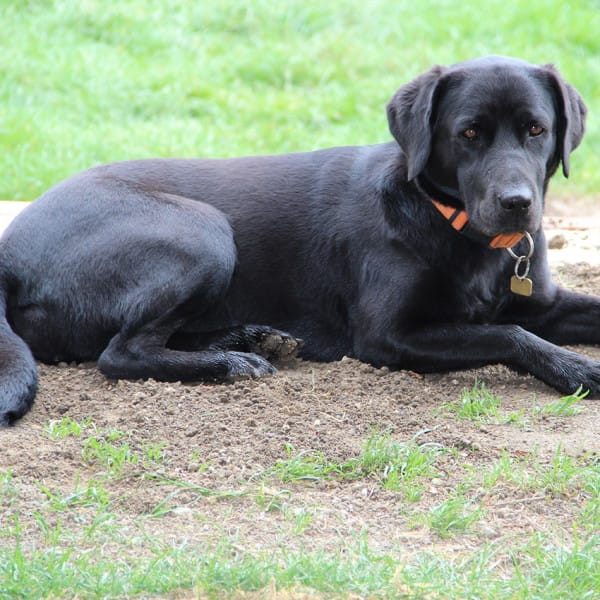
\includegraphics[width=0.6\textwidth]{black-lab-dog}
      \end{figure}
    \end{column}%
  \end{columns}
\end{frame}


\section{Logically real}


\begin{frame}{Concepts and Judgement}
\begin{figure}
  \centering
  \begin{columns}
    \column{0.5\textwidth}
    \centering
    \caption {Intentional form}
    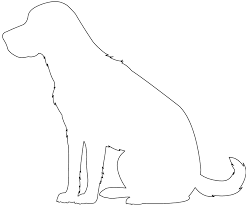
\includegraphics[width=0.99\textwidth]{dog-outline}
    \column{0.5\textwidth}
    \centering
    \caption {Swappable attributes}
    
\includegraphics[width=0.99\textwidth]{black}
  \end{columns}
\end{figure}
\end{frame}


\section{Ontologically real}


\begin{frame}[fragile]{Experimental data}
  \begin{columns}[T] % align columns
    %% \begin{column}{0.3\textwidth}
    %% \end{column}%
    %% \hfill%
    \begin{column}{0.99\textwidth}
      \begin{figure}[H]
        \centering
        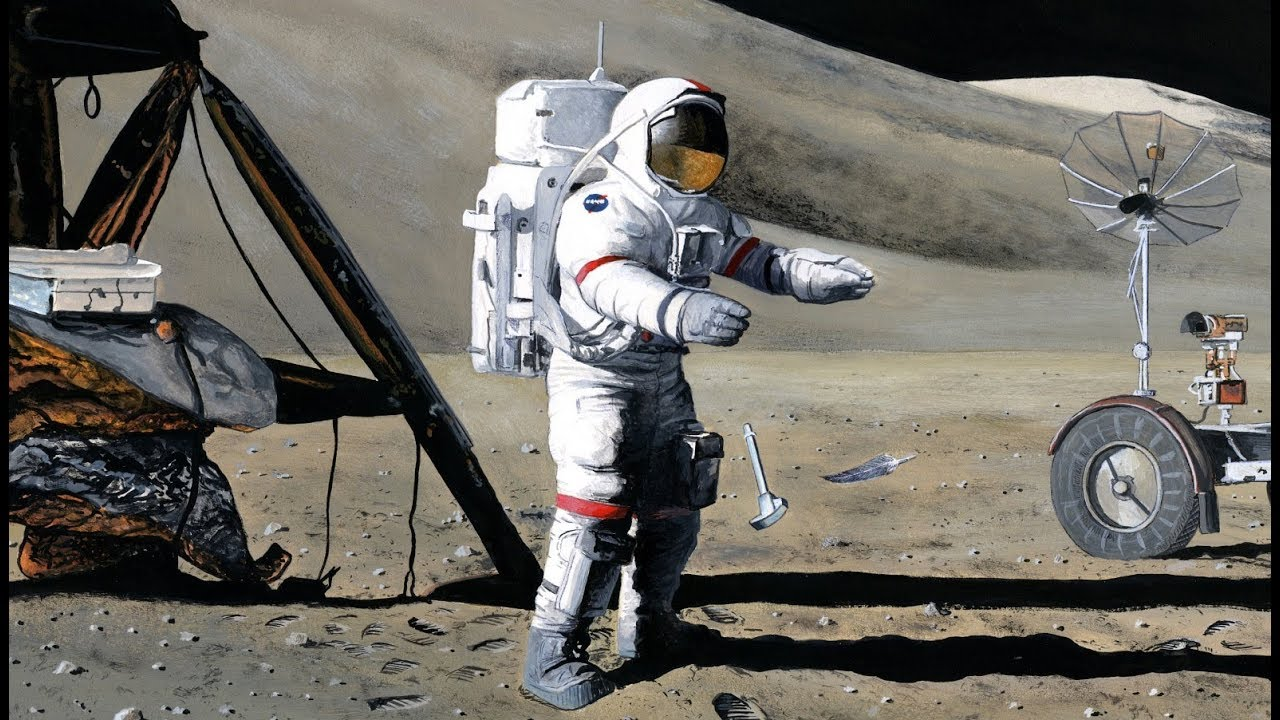
\includegraphics[width=0.95\textwidth]{gravity}
      \end{figure}
    \end{column}%
  \end{columns}
\end{frame}


\section{Logically real}


\begin{frame}{Descriptive, not operative, laws}
  \begin{columns}[T] % align columns
    %% \begin{column}{0.3\textwidth}
    %% \end{column}%
    %% \hfill%
    \begin{column}{0.99\textwidth}
      \begin{figure}[H]
        \centering
        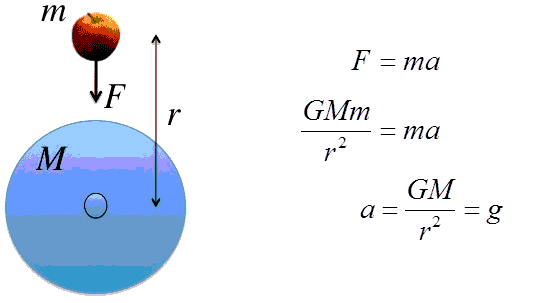
\includegraphics[width=0.8\textwidth]{gravitation-law}
      \end{figure}
    \end{column}%
  \end{columns}
\end{frame}


\section{More logical than ontological}


\begin{frame}[fragile]{Music produced}
  \begin{columns}[T] % align columns
    %% \begin{column}{0.3\textwidth}
    %% \end{column}%
    %% \hfill%
    \begin{column}{0.99\textwidth}
      \begin{figure}[H]
        \centering
        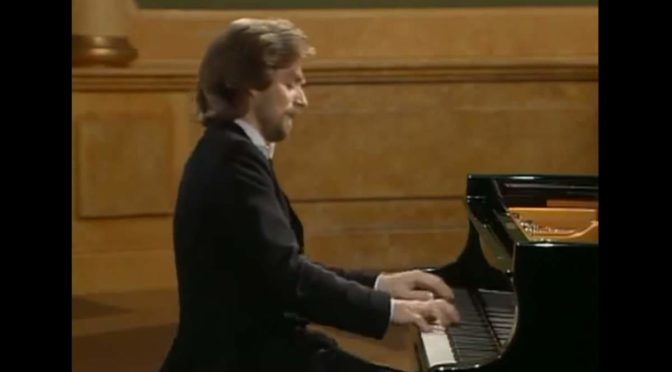
\includegraphics[width=0.95\textwidth]{zimerman}
      \end{figure}
    \end{column}%
  \end{columns}
\end{frame}

\begin{frame}[fragile]{Music's correspondence}
  \begin{itemize}
      \item Art imitates nature. \vspace{5mm}
  \item Music, an art, is not distinct from us like a cat or dog is, as it does not imitate something distinct from us.\vspace{5mm}
    \item Rather, it imitates the passions themselves, those powers within us that move us to action.\vspace{5mm}
  \end{itemize}
\end{frame}


\begin{frame}[fragile]{Music's parts}
  \begin{columns}[T] % align columns
    %% \begin{column}{0.3\textwidth}
    %% \end{column}%
    %% \hfill%
    \begin{column}{0.99\textwidth}
      \begin{figure}[H]
        \centering
        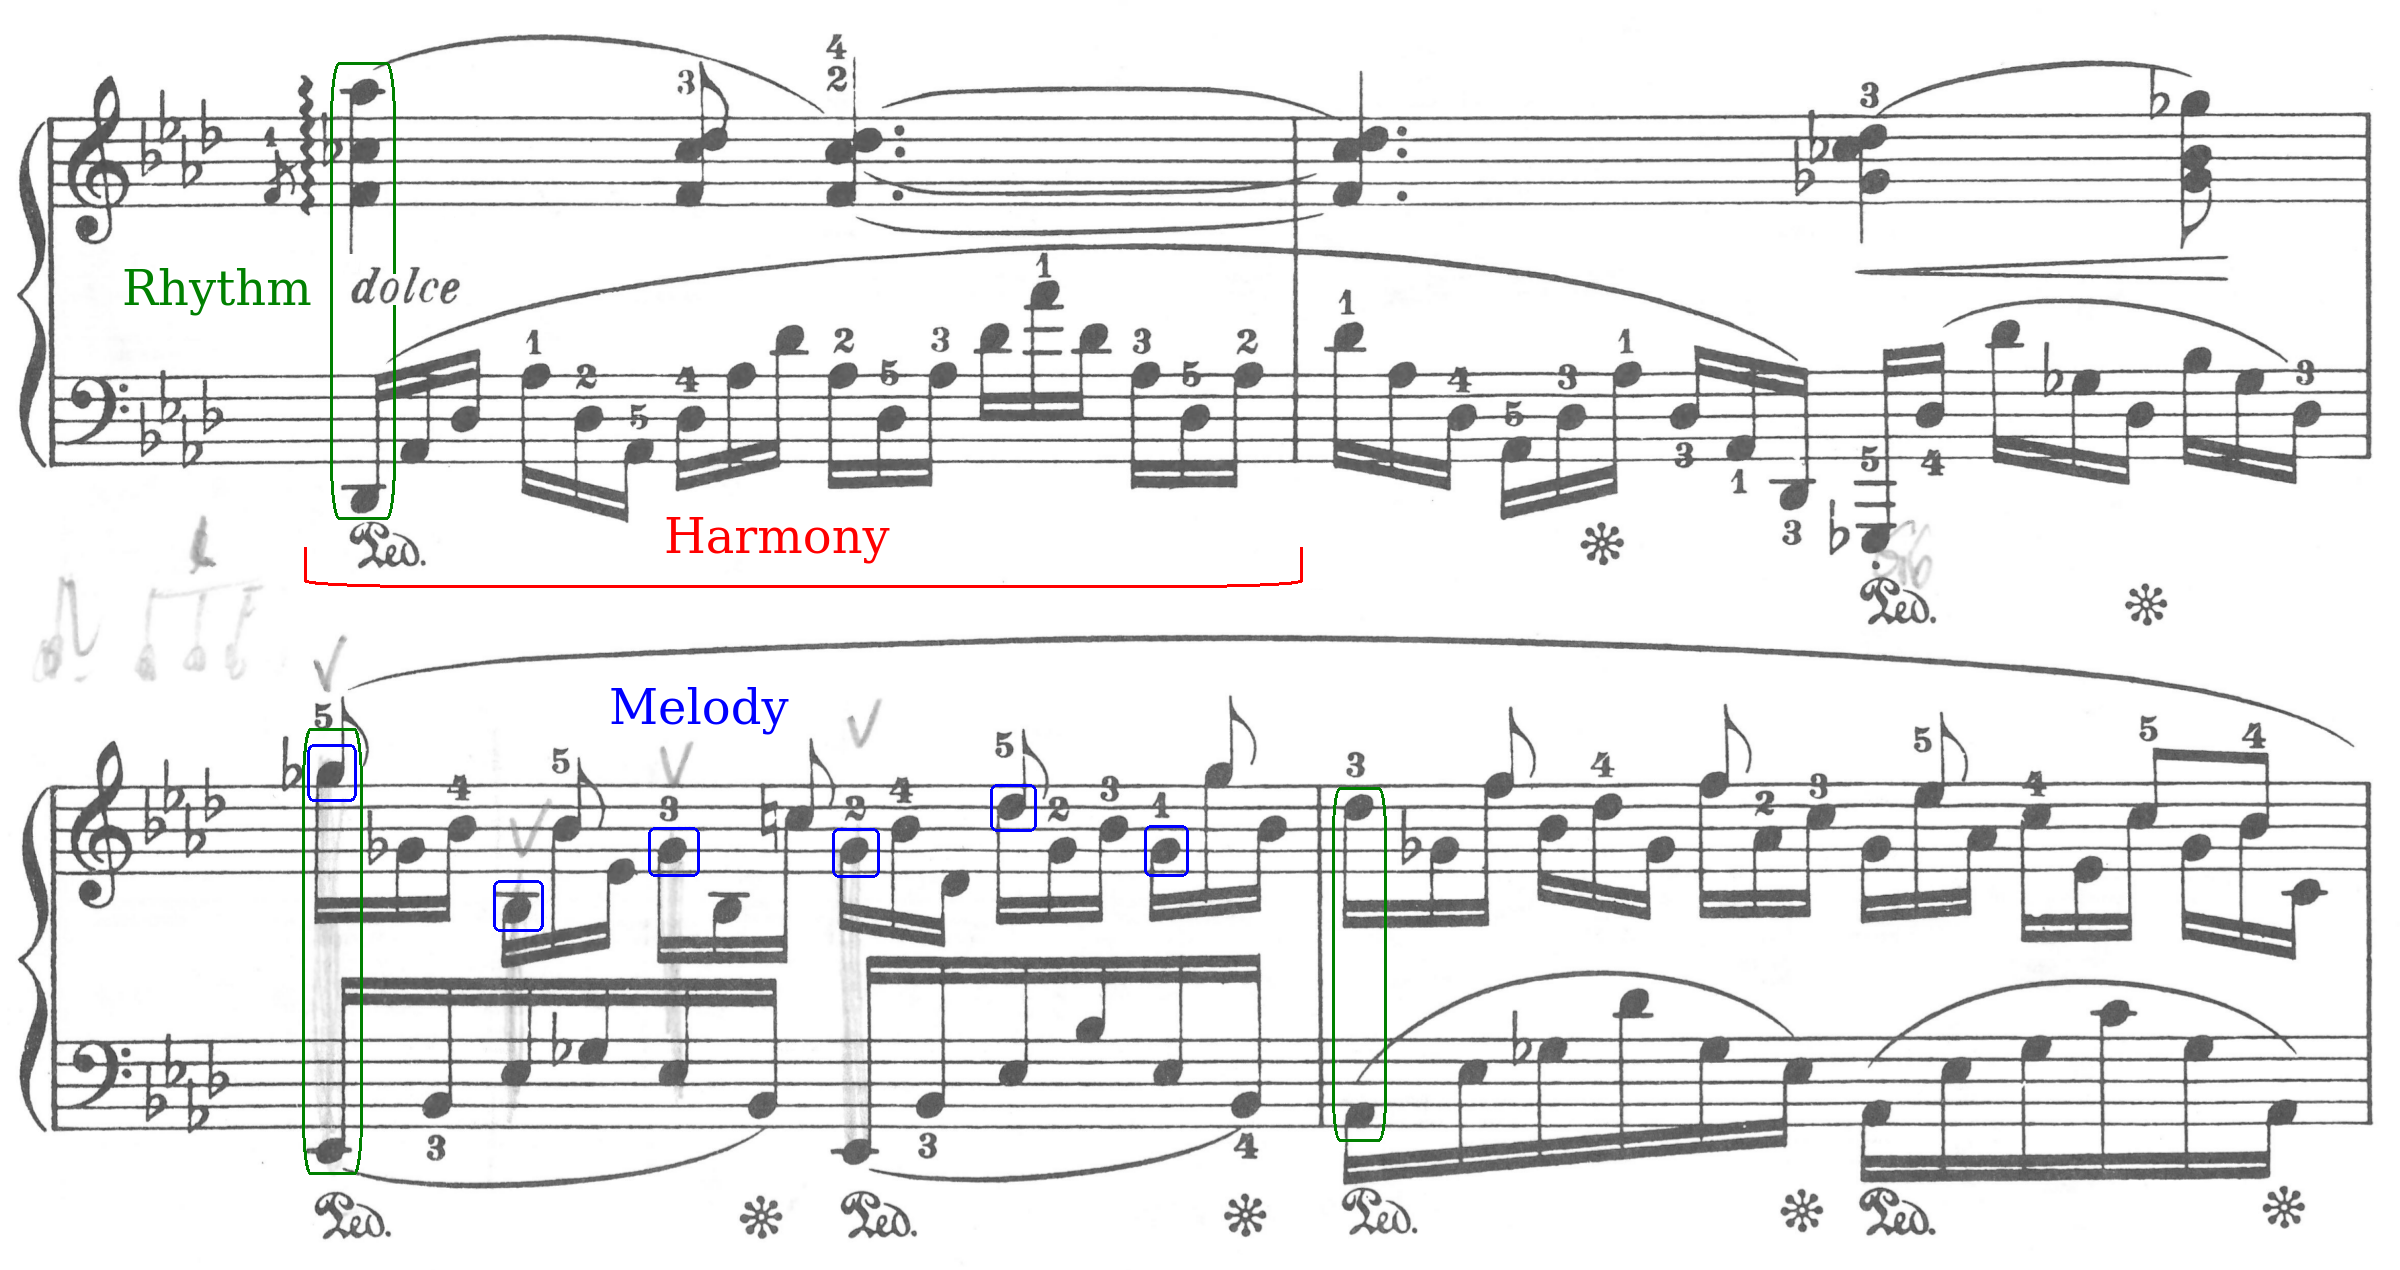
\includegraphics[width=0.99\textwidth]{chopin-ballade-rhm}
      \end{figure}
    \end{column}%
  \end{columns}
\end{frame}


\begin{frame}[fragile]{\emph{We} see properties shining together}
  \begin{itemize}
  \item Melody is simple --- the intellect grasps unities (essences).\vspace{5mm}
  \item Harmony accompanies melody --- the will desires the good presented by the intellect. \vspace{5mm}
  \item Rhythm sustains both --- the body operates at a tempo (breathing, heartbeat, etc). \vspace{5mm}
  \item {\ldots} But music is the whole thing.
  \end{itemize}
\end{frame}



\section{Intrinsic immateriality}


\begin{frame}[fragile]{Abstraction produces a concept}
  \begin{columns}[T] % align columns
    %% \begin{column}{0.3\textwidth}
    %% \end{column}%
    %% \hfill%
    \begin{column}{0.99\textwidth}
      \begin{figure}[H]
        \centering
        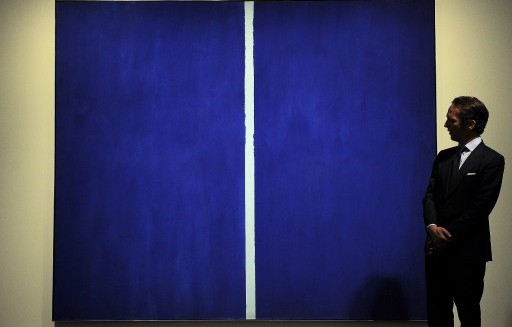
\includegraphics[width=0.9\textwidth]{abstract}
      \end{figure}
    \end{column}%
  \end{columns}
\end{frame}


\begin{frame}[fragile]{Semantically simple --- no parts}
  \begin{columns}[T] % align columns
    %% \begin{column}{0.3\textwidth}
    %% \end{column}%
    %% \hfill%
    \begin{column}{0.99\textwidth}
      \begin{figure}[H]
        \centering
        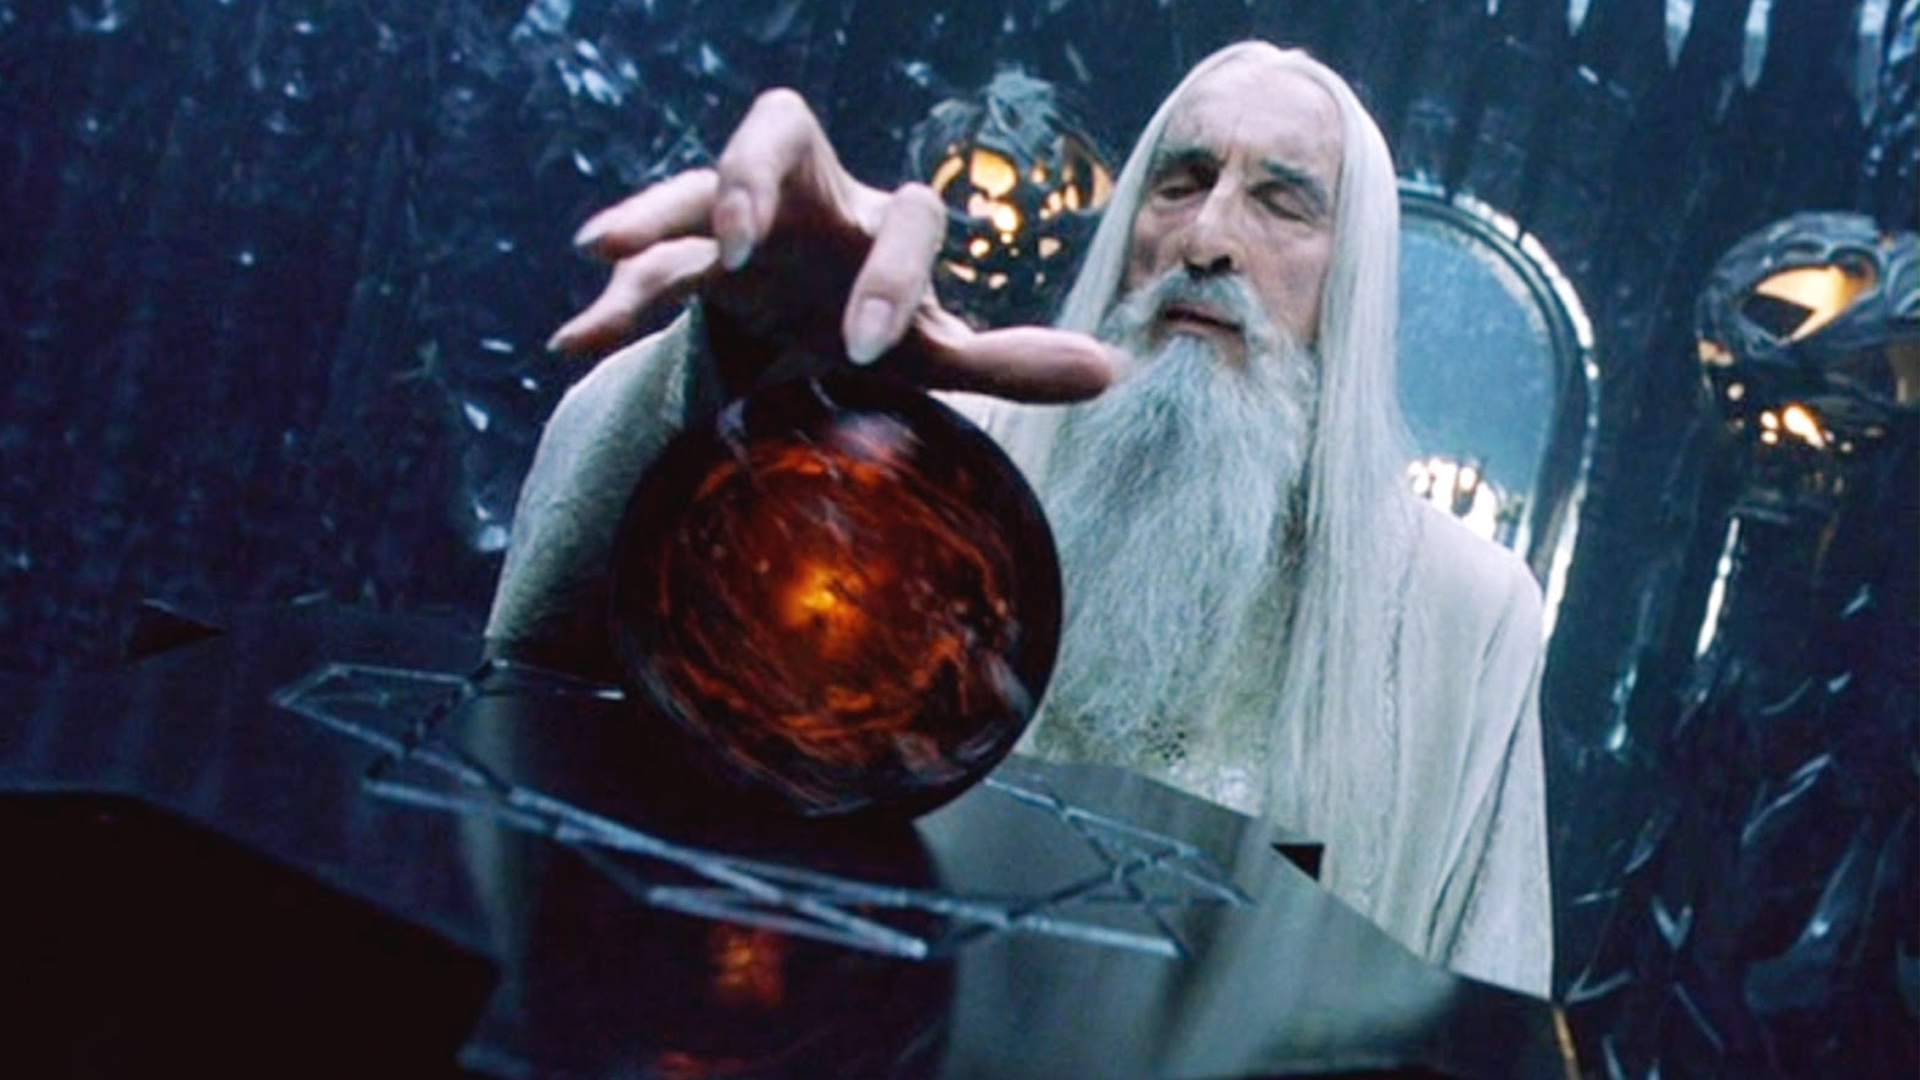
\includegraphics[width=0.9\textwidth]{crystal-ball}
      \end{figure}
    \end{column}%
  \end{columns}
\end{frame}


\begin{frame}[fragile]{Where is `unity' stored?}
  \begin{columns}[T] % align columns
    %% \begin{column}{0.3\textwidth}
    %% \end{column}%
    %% \hfill%
    \begin{column}{0.99\textwidth}
      \begin{figure}[H]
        \centering
        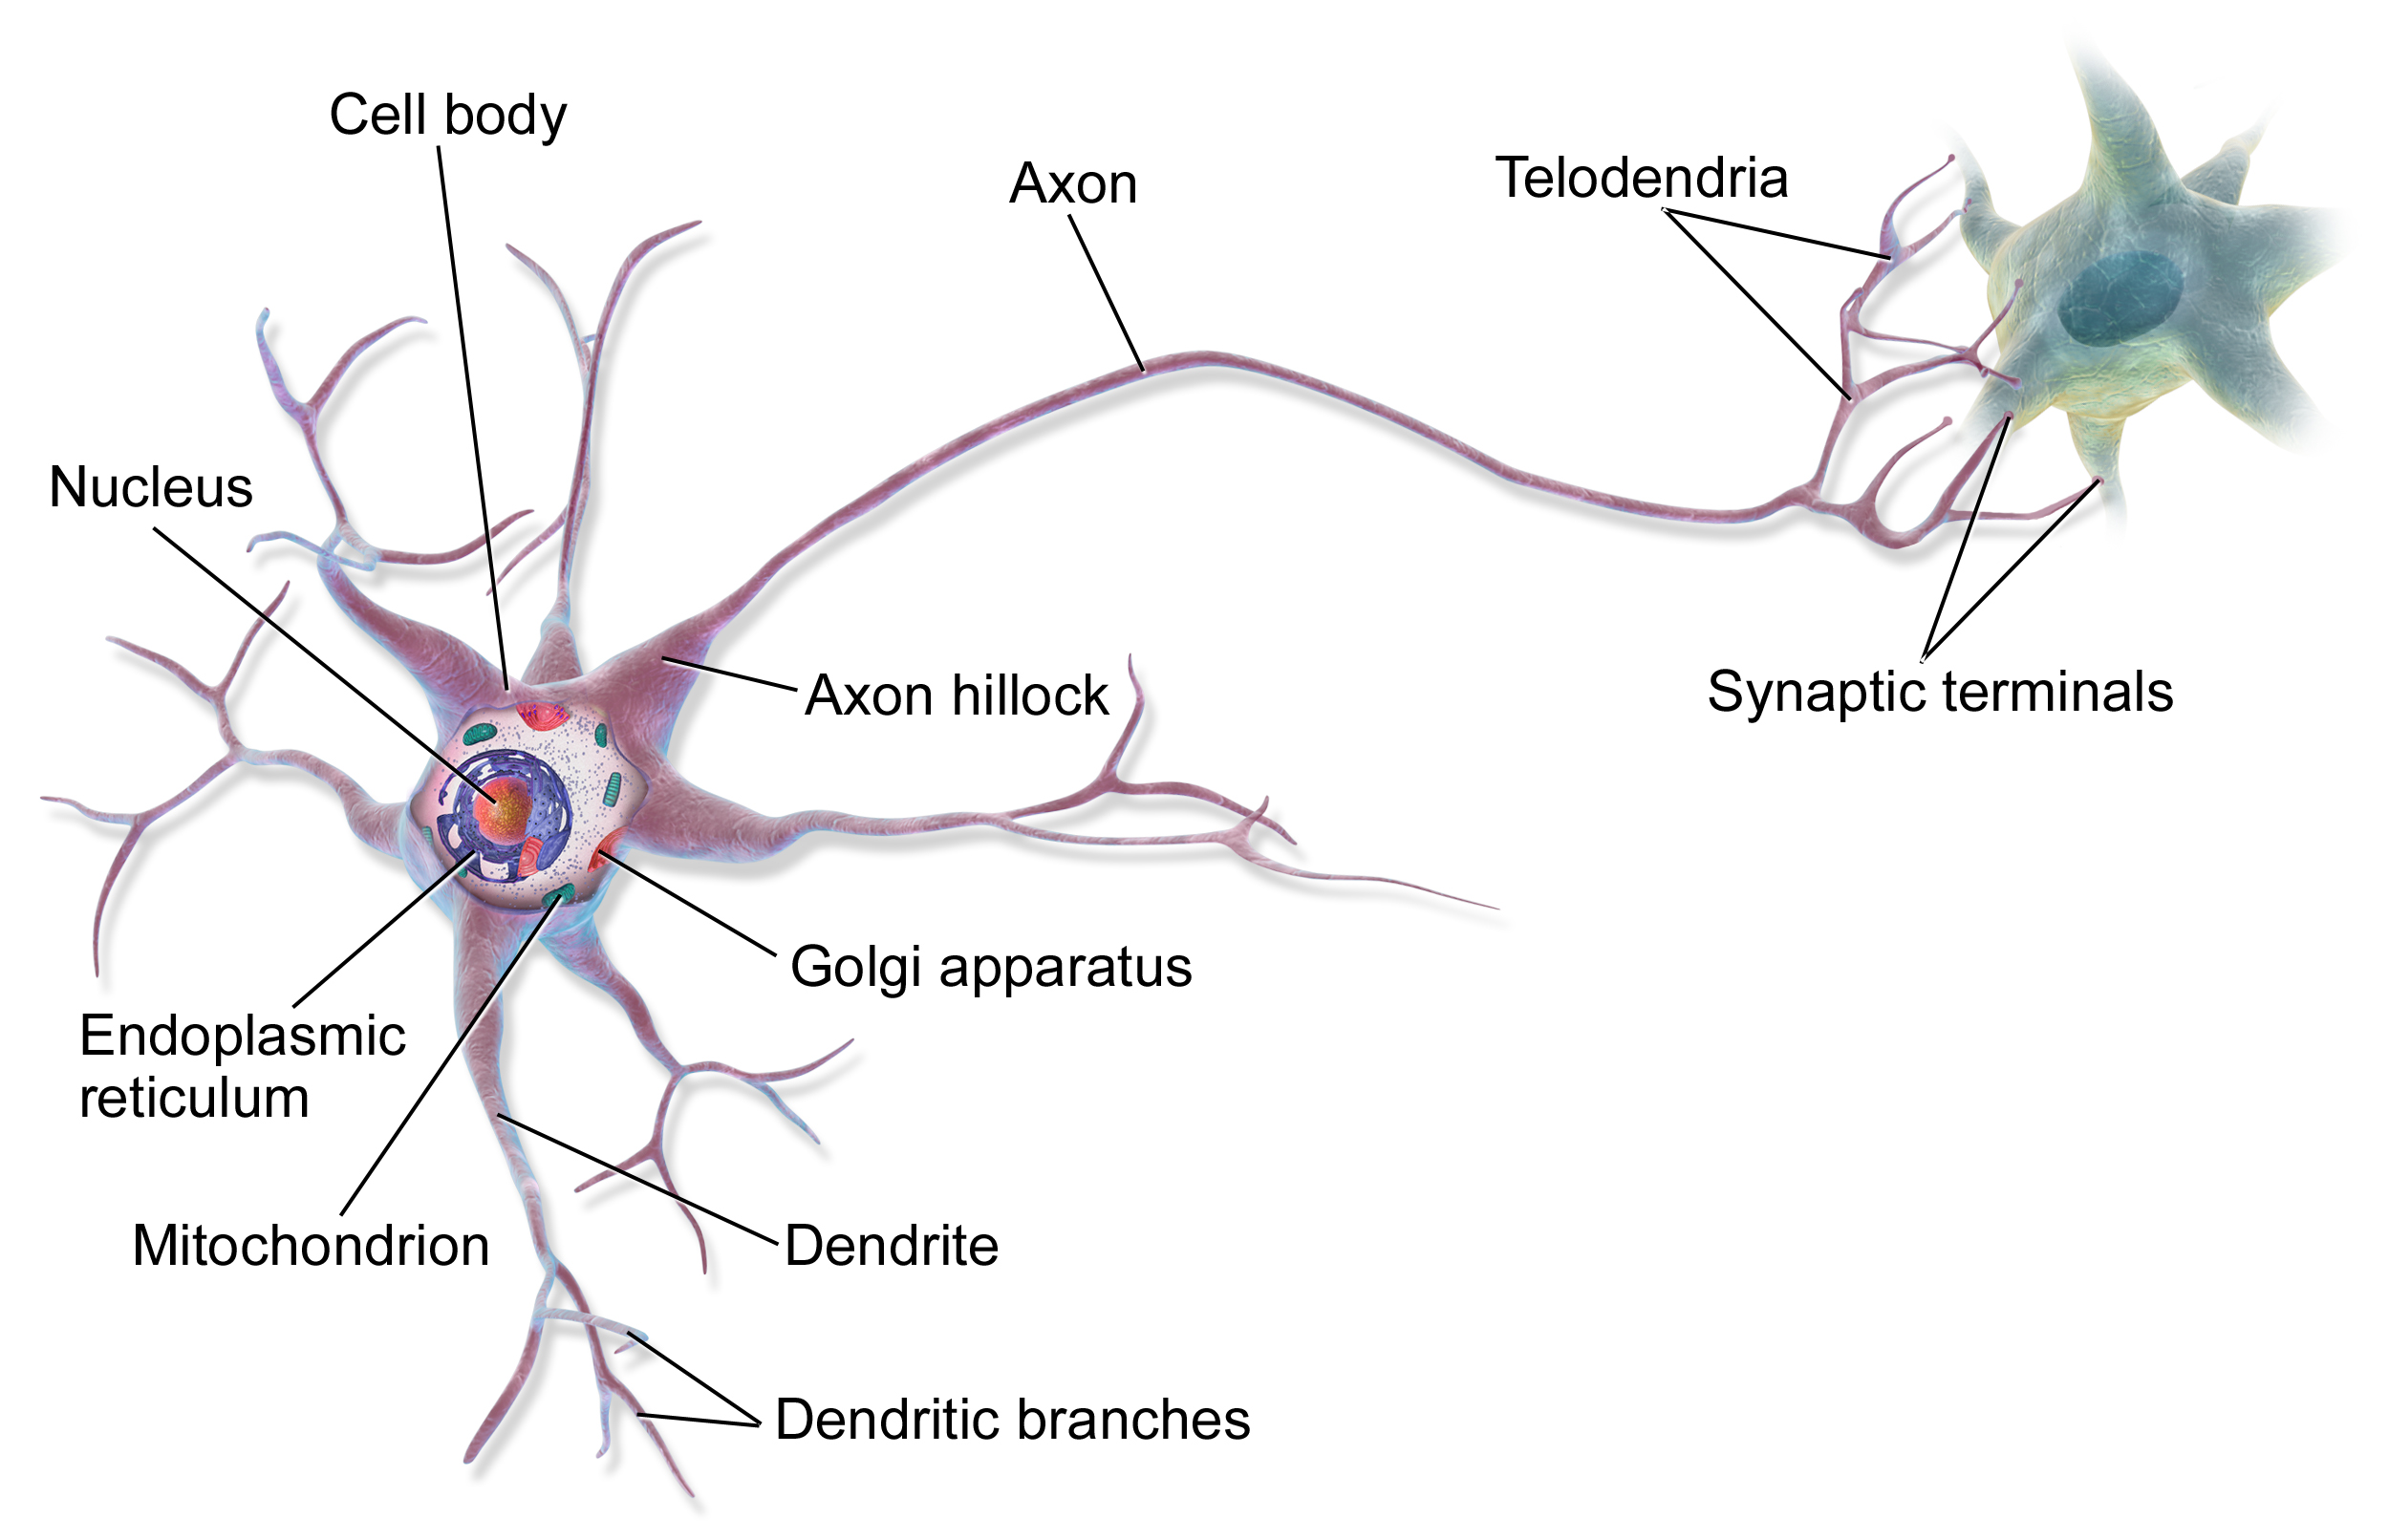
\includegraphics[width=0.9\textwidth]{neuron}
      \end{figure}
    \end{column}%
  \end{columns}
\end{frame}


\begin{frame}{Act of the intellect}
  \begin{columns}[T] % align columns
    \begin{column}{0.5\textwidth}
\textbf{1. Simple Apprehension}
  \begin{itemize}
  \item Intention: \emph{Essences or Natures}
  \item Product: \emph{Concept}
  \item Characteristics: \emph{Clear or Unclear}
  \item Question: \emph{What?}
  \end{itemize}

  ~

\textbf{2. Judgement}
  \begin{itemize}
  \item Intention: \emph{Acts of Existence}
  \item Product: \emph{Proposition}
  \item Characteristic: \emph{True or False}
  \item Question: \emph{Whether?}
  \end{itemize}
    \end{column}%
    %% \hfill%
    \begin{column}{0.5\textwidth}
\textbf{3. Reasoning}
  \begin{itemize}
  \item Intention: \emph{Causes or Reasons}
  \item Product: \emph{Argument}
  \item Characteristics: \emph{Valid or Invalid}
  \item Question: \emph{Why?}
  \end{itemize}
    \end{column}%
  \end{columns}
\end{frame}


\begin{frame}[fragile]{Considerations}
  \begin{itemize}
  \item `Real' has at least two senses --- out there, and in the mind.\vspace{5mm}
  \item The intellect analyses --- splits unities into conceptual differences.\vspace{5mm}
  \item The intellect synthesises --- unites conceptual differences into a whole.\vspace{5mm}
  \item Unity, truth and goodness are abstract --- likewise rhythm, harmony and melody.\vspace{5mm}
  \item The intellect synthesises this as beauty --- likewise as music.\vspace{5mm}
  \end{itemize}
\end{frame}


\begin{frame}[plain]
  \titlepage
\end{frame}

\end{document}
